\section{Overview}

\begin{enumerate}

\item A probabilistic view of the world lies behind everything: in particular, any conclusion based on data. But also quantum physics, perception, machine learning, etc.
\item Every statement you can make about the world, every observable outcome of any process, any data you can collect; all of these can be thought of as ``random variables​''.

\item {\bf Why would we be interested in learning about this? What can we do with this?}
  \begin{enumerate}
  \item Form a conclusion about something unknown (Do I have Covid? Is that a leaf I see in front of me? What species of bird is that singing? What is this person saying?)
  \item Make a decision (What policy should this government choose? Should this self-driving car come to an abrupt stop right now? Should I as a soldier attempt to kill that man?)
  \item Form a conclusion about causality (Do cell phones cause cancer? Did the dinosaurs go extinct because of a meteor strike?)
  \end{enumerate}

\item {\bf Overview}
  \begin{enumerate}
  \item The idea of a \defn{random variable​}
  \item The idea of a \defn{joint probability distribution}
  \item Network diagrams, correlation/independence
  \item How should we form conclusions about unknowns?
    \begin{enumerate}
    \item The idea of a \defn{probability model} and a \defn{generative process}
    \item Updating beliefs after making observations
    \item What is ``statistics​''? What is ``theory​''?
    \end{enumerate}
  \item How should we make decisions?
  \item How should we form conclusions about causality?
  \item Quantum physics (?)
  \end{enumerate}

\item {\bf 1. Random variables}
  \begin{enumerate}
  \item The simplest example is the coin flip.
  \item Bar plot of probability
  \item Reality is somehow coming up with things in proportion to those two probability masses.
  \item Summaries of RVs: mean, etc (?)
  \end{enumerate}

\item {\bf 2. Joint probability distributions}
  \begin{enumerate}
  \item But we need to be able to think about the probability of many things simultaneously, or of a single complex thing.
  \item Example of two uncorrelated things. How do we picture this? Diagram of two bar plots next to each other.
  \item That's not quite right though. Our outcomes are now ``tuples​''
  \item Diagram of 2D barplot.
  \item But what if we have 3 things? Or millions of things?
  \item Spreadsheet format: list all possible tuples using the first d columns, enter probability of that tuple in the final column
  \end{enumerate}

\item 3. {\bf Network diagrams, correlation}

\item 4. {\bf How should we form conclusions about unknowns?}
  \begin{enumerate}
  \item The simplest way to think about this, which is always a valid way to think about it, is the Bayesian way:
    \begin{enumerate}
    \item Agree on the joint probability distribution of all the unknowns (including hypotheses, parameters, and observable data values)
    \item It might be clearest to represent it as a network diagram
    \item This is called a ``model​'' (or ``statistical model​'')
    \item Make some measurements of the observable data values
    \item Look at how the probabilities in the model have changed
    \end{enumerate}
  \item What about ``hypothesis tests​'' and ``p-values​''?
    \begin{enumerate}
    \item Identify a null hypothesis
    \item Write down the model (joint probability distribution) as before, but this time with all the probabilities
      conditional on the null hypothesis being true.
    \item Observe some data
    \item Use the model to write down the probability that the model would spit out the data that you observed, or
      data more extreme than what you observed (here ``more extreme​'' means less consistent with the null
      hypothesis).
    \item This probability is known as a \defn{p-value}. If it is very small we conclude that the null hypothesis is unlikely
      to be true: i.e. it seems more likely that the data set was spat out by some other model, not the model
      we have with the hypothesis fixed at the null hypothesis.
    \end{enumerate}
  \end{enumerate}
\end{enumerate}




TODO:

\begin{itemize}
\item model as generative procedure
\item Nature/reality as generative procedure
\item What does it mean to talk of a generative procedure for a non-observable?
\item philosophy: according to frequentists, percent of Amazon remaining in 2035 is whatever it is, it's not random
\end{itemize}




\section{Random variables}

There are basically two things to know about a random variable:
\begin{enumerate}
\item It has some fixed range of possible values. In our example: heads and tails.
\item Each value has a probability associated with it.
\end{enumerate}

It's usually best to start off with a very simple example. The simplest possible random variable would have
just one possible value. But the usual word for one of those is a ``fact​'', since there is no uncertainty about
its value. So, let's start with a random variable with two possible values.



What should the example be here? We want something which feels very much like reality has ``picked​'' one of the
two values randomly. And we want something that can be part of a correlated 2-tuple.

\begin{enumerate}
\item heads/tails?
\item sex of a baby?
\item radioactive emissions?
\item shooting stars?
\end{enumerate}


There are basically two things to know about a random variable:
\begin{enumerate}
\item It has some fixed range of possible values. In our example: heads and tails.
\item Each value has a probability associated with it.
\end{enumerate}


The picture we should have in mind is a simple one:

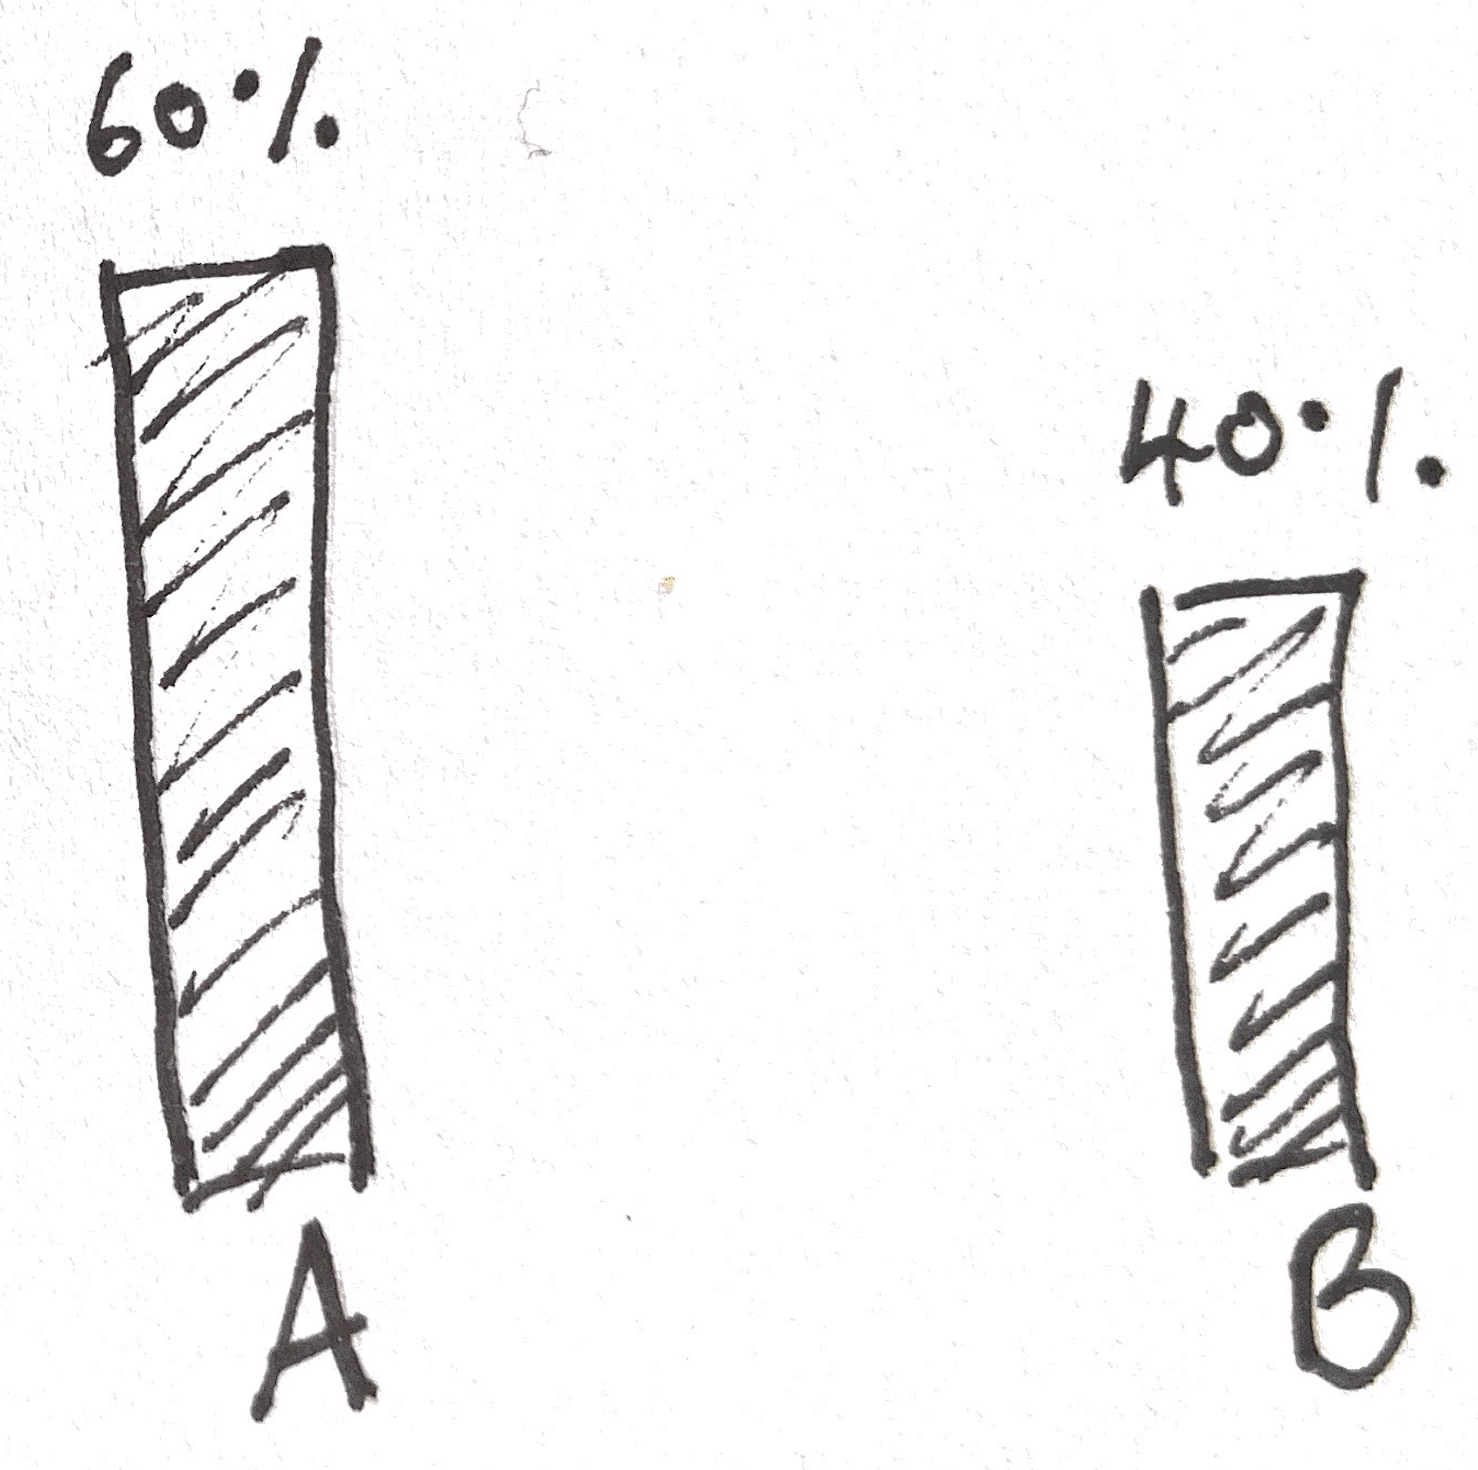
\includegraphics[width=400pt]{img/statistics-and-machine-learning--introduction--overview--random-variables-8b8d.png}



Let's try to think of this as a very purely random phenomenon. It's not easy: if you take most examples that
someone might put forward and think about them, you end up concluding that to a large extent it's not ``really​''
random, it's more that we're in ignorance of what exactly is going on. Taking the coin flip as an example,
basically no-one is going to try to precisely characterise the impact of your finger nail with the surface of
the coin, and the precise shape and density of the coin etc to be able to do the physics calculations. Instead
we just say: it's approximately 50:50 which way it will land.

A better example might be a small lump of weakly radioactive rock. You sit there with a Geiger counter and
suitable protective clothing and watch the Geiger counter display for 10 seconds. Is there an emission during
that time or not? It's yes or no. We don't care what the probabilities of the two possibilities are but the
point is that this feels really quite random. Even if we could observe what's going on at a subatomic level
physicists tell us that at sufficiently fine levels of detail they also throw up their hands and say it appears
to be truly random.






This is an attempt to explain the basic ideas behind some commonly-heard jargon such as: ``statistics​'', ``machine
learning​'', ``artificial intelligence​'', ``data science​'', ``statistical inference​​​''.

Basically, all those areas have to do with how we use observations to shape our beliefs about the world and make decisions. That's extremely broad. For example, it includes
\begin{itemize}
\item Observing some coin tosses and forming a belief about whether the coin is biased.
\item Observing the results of an experiment and updating your beliefs regarding whatever was being investigated.
\item Hearing a bird and forming a belief about what species it is.
\item Observing the data from a test for a disease, and forming a belief about whether the patient has the disease.
\item Observing some economic data and forming a belief about how the economy will behave in the near future.
\item Observing some data about a society and deciding the measures that its government should take.
\item Observing some fossils and forming beliefs about how life evolved on Earth in the distant past.
\item Photons of light hitting your retina, and your brain forming beliefs about what it sees and what to do.
\item The same thing, but for an artificial retina feeding its data to a computer program (e.g. a self-driving car).
\end{itemize}
Scientists, engineers and mathematicians think about all these disparate processes using the same basic conceptual framework, which is based on probability. The central object that one thinks about in probability is known as a "random variable". This is basically what it sounds like: it's a thing whose value may not be known with certainty.

The classic first example of a random variable is "what I get when I toss this coin". That example certainly captures the basics: the random variable has two possible states, and there's a certain probability associated with each one. However, the concept of a random variable is much more widely applicable than that. Let's go back to the definition above: "a thing whose value may not be known with certainty". There are a lot of different things that we may not know with certainty; here are some examples:
\begin{itemize}
\item What I get when I toss this coin
\item Who will win the election
\item Whether Schrödinger's cat is still alive when I open its box
\item The height of the next person I pass in the street
\item The percentage of the Amazon rainforest that will remain in 2035
\item Whether we are living in a computer simulation
\end{itemize}
Some of those are "an outcome" whereas some are more like "an answer to a question", but in either case there is uncertainty. The examples are chosen to illustrate the broad scope of the concept but note that they all still fit the same conceptual framework as the coin toss, i.e. in each case we can ask the same questions as we asked about the coins: How many different possibilities are there? What are the numerical probabilities associated with the different values? Of course, the number of possible values might be infinite, and it may be very hard to say anything about their probabilities, but they are still "random variables" despite those challenges:

\begin{table}[h!]
  \centering
  \begin{tabular}{|l|l|l|}
    \hline
    {\bf Outcome/Question}                  & {\bf Possible values} & {\bf Probability distribution} \\
    \hline
What I get when I toss this coin             & Heads, Tails & 50\%: 50\% if the coin is fair\\
    \hline
Who will win the election                     & Biden or Trump & Could be estimated from polling results\\
    \hline
Whether Schrödinger's cat is                 & Yes or No & Could be calculated from physics theory \\
still alive when I open its box                &              &  if the set-up were simple enough \\
    \hline
The height of the next person                & Infinitely many values & Could be estimated by measuring  \\
I pass in the street                               & between, say,  & the heights of a large sample  \\
                                                       & 3ft and 8ft & of the population \\
    \hline
The percentage of the Amazon rainforest & Infinitely many values & Could be roughly estimated but  \\
that will remain in 2035                       & between 0 and 100 & would be uncertain and subject to disagreement \\
    \hline
Whether we are living                          & Yes or No & Hard to know how to estimate,  \\
in a computer simulation                      &            & would be uncertain and subject to disagreement \\
    \hline
  \end{tabular}
\end{table}

In the right-hand column, labeled "Probability distribution", most of the entries say "could be estimated" or
have caveats. The fact is that is it often debatable what probabilities should be assigned to different
outcomes. However, it is also necessary that we take a stab at it if we are to be able to update our beliefs or
decisions in light of observed data, and this assignment of probabilities to the possible outcomes has a name
that one comes across fairly frequently in non-technical writing: it is known as a "model". Of course, if we're
wrong about the model, our updated beliefs/decisions may be inappropriate.


To continue to make things concrete, here are some of the scenarios that I listed above with the random variables explicitly identified:

\begin{table}[h!]
  \centering
  \begin{tabular}{|l|l|}
    \hline
    {\bf Random variable being observed} & {\bf Random variable we form beliefs about} \\
    \hline
    The frequencies and spatial pattern of photons  & The identities of the objects in the scene in front of me \\
    hitting my retina & \\
    \hline
    A sequence of heads and tails  & Whether the coin is biased \\
    \hline
    An audio signal                    & Whether it is a bird and if so what species \\
    \hline
    A sequence of values of some economic statistic & What the economy will do \\
    over some period of time   & \\
    \hline
  \end{tabular}
\end{table}

Notice that a random variable can be very simple (the outcome of tossing a coin once), or very complex (an audio signal over some period of time, i.e. at each of many sampled time points, a list of all the audio frequencies that are present and their intensities). The complex random variable is made up of many components, each of which could be considered a random variable in its own right. But none of that changes the basic idea: a random variable is a thing (an outcome, or an answer to a question) about which we are uncertain.





\section{Bayesian Networks}


Consider some collection of random variables $X_1, \ldots, X_n$. We can think of them as vertices of a graph:

\begin{align*}
\begin{tikzpicture}
  \graph[math nodes, spring layout, edges=white]{X_1 -> {X_2, X_3, X_4}, X_2 -> {X_3, X_4}, X_3 -> {X_4}, X_4};
\end{tikzpicture}
\end{align*}


If we know some of the conditional distributions, then we can pick an ordering and factorise the joint
distribution:
\begin{align*}
  \p(X_1, X_2, X_3, X_4) = \p(X_1) \p(X_2|X_1) \p(X_3|X_2, X_1) \p(X_4|X_3, X_2, X_1).
\end{align*}

When $X_1$ and $X_2$ are not independent, we draw a directed edge from $X_1$ to $X_2$ to refer to the conditional probability distribution $\p(X_2|X_1)$. The graph corresponding to the above factorisation is
\begin{align*}
\begin{tikzpicture}
  \graph[math nodes, spring layout]{X_1 -> {X_2, X_3, X_4}, X_2 -> {X_3, X_4}, X_3 -> {X_4}, X_4};
\end{tikzpicture}
\end{align*}

That graph is complete (contains every possible edge). However, if some variables are conditionally independent of others, then we can get rid of some of the edges.

{\bf Example}: will my team win this football match?
Let:
\begin{itemize}[label=$\circ$]
\item $X_1 = ~$ is our best player playing?
\item $X_2 = ~$ are we playing at home?
\item $X_3 = ~$ number of goals each teams scores in the match
\item $X_4 = ~$ do we win the match?
\end{itemize}

Notice that there is now some conditional independence:
\begin{itemize}
\item The number of goals scored by both teams is influenced by whether our best player is playing and whether it's a home game.
\item For the sake of argument, let's say that whether we're playing at home doesn't influence whether our best player is playing.
\item Whether we win the match is determined by the number of goals scored: if we know the number of goals scored then knowing whether our best player was playing, or whether it was a home game, doesn't provide any further information about whether we won the match.
\end{itemize}
The conditional independence simplifies the graph:

\begin{table}[!h]
  \centering
  \begin{tabular}{|c|c|}
    All arrows included & Delete arrows between independent nodes\\
    \hline
    \begin{tikzpicture}\graph[math nodes, spring layout, edges=very thick]{X_1 -> {X_2, X_3, X_4}, X_2 -> {X_3, X_4}, X_3 -> {X_4}, X_4};\end{tikzpicture}
    &\begin{tikzpicture}\graph[math nodes, tree layout, edges=very thick]{X_1 -> {X_3}, X_2 -> {X_3}, X_3 -> {X_4}, X_4};\end{tikzpicture}
  \end{tabular}
\end{table}


So what is this network diagram really? It represents the probability distribution of the compound random variable $(X_1, X_2, X_3, X_4)$ . In other words, it specifies a generative procedure which spits out compound values of the form $(x_1, x_2, x_3, x_4)$. The generative procedure is
\begin{enumerate}
\item Pick whether or not our best player is playing according to the yes/no probabilities for $X_1$.
\item Pick whether we are playing at home (50:50 if it's a league match and we don't know the date).
\item Conditional on those two things, generate the score in the match (Nature can do this by just moving time forwards, but a human would have to do a lot of work to be able to claim that they could simulate match scores from anything like the true probability distribution.)
\item Finally, whether we win (yes/no) is a deterministic function of the score (i.e. conditional on the score, whether we win can be thought of as a random variable with no uncertainty).
\end{enumerate}
The first few values generated by that generative procedure might be

\begin{verbatim}
(yes, no,  1-2, yes)
(no,  no,  1-1, no)
(yes, yes, 2-1, yes)
        ...
\end{verbatim}

Each time a random value is generated from the probability distribution, we can imagine the component values appearing at the corresponding nodes of the graph:

\begin{table}[h!]
  \centering
  \begin{tabular}{|c|c|}
    \hline
    & \\
    (yes, no,  1-2, yes)
    &
      \adjustbox{valign=m}{\begin{tikzpicture}\graph[tree layout, edges=very thick]{X_1 [as=Best player plays] -> {X_3 [as=Score 1-2]}, X_2 [as=Away game] -> {X_3}, X_3 -> {X_4 [as=Win]}, X_4};\end{tikzpicture}} \\
    & \\
    \hline
    & \\
    (No, No ,  1-1, No)
    &
    \adjustbox{valign=m}{\begin{tikzpicture}\graph[tree layout, edges=very thick]{X_1 [as=Best player doesn't play] -> {X_3 [as=Score 1-1]}, X_2 [as=Away game] -> {X_3}, X_3 -> {X_4 [as=Draw]}, X_4};\end{tikzpicture}} \\
    & \\
    \hline
    & \\
    (Yes, Yes,  4-1, Yes)
    &
    \adjustbox{valign=m}{\begin{tikzpicture}\graph[tree layout, edges=very thick]{X_1 [as=Best player plays] -> {X_3 [as=Score 4-1]}, X_2 [as=Home game] -> {X_3}, X_3 -> {X_4 [as=Win]}, X_4};\end{tikzpicture}} \\
    & \\
    \hline
  \end{tabular}
  \caption{Examples of random values generated from the football model}
\end{table}


%